%%%%%%%%%%%%%%%%%%%%%%%%%%%%%%%%%%%%%%%%%%%%%%%%%%%%%%%%%%%%%%%%%%%%%%
% writeLaTeX Example: Academic Paper Template
%
% Source: http://www.writelatex.com
% 
% Feel free to distribute this example, but please keep the referral
% to writelatex.com
% 
%%%%%%%%%%%%%%%%%%%%%%%%%%%%%%%%%%%%%%%%%%%%%%%%%%%%%%%%%%%%

\documentclass[twocolumn,showpacs,%
  nofootinbib,aps,superscriptaddress,%
  eqsecnum,prd,notitlepage,showkeys,10pt]{revtex4-1}

\usepackage{natbib}
% \usepackage[square,numbers]{natbib} % TODO
\bibliographystyle{unsrtnat}

% displays all math in sans-serif font TODO  
\usepackage[cm]{sfmath}
  
\usepackage{graphicx}
\graphicspath{ {images/} }

\usepackage{listings}
\lstset{
basicstyle=\small\ttfamily,
%basicstyle=\ttfamily,
columns=flexible,
breaklines=true
}
%\lstset{language=Coq}

\usepackage [english]{babel}
\usepackage [autostyle, english = american]{csquotes}
\MakeOuterQuote{"}

\usepackage{amssymb}
\usepackage{amsmath}
\usepackage{graphicx}
\usepackage{dcolumn}
\usepackage{hyperref}

% \newcommand{name}[num]{definition}
\newcommand{\eqn}[1] {\begin{gather*}#1\end{gather*}}
\newcommand{\spc} {\textrm{ }}
\newcommand{\s} {\textrm{ }}

\begin{document}

\title{Formally proving equivalence between abstract and concrete specifications of HMAC}
\author{Katherine Ye, advised by Andrew Appel}
\affiliation{Princeton University}

\begin{abstract}
The OpenSSL implementation of HMAC has been proven to correctly implement a concrete specification. HMAC uses SHA-256 as its hash function, and the SHA-256 program has also been proven to correctly implement its specification. At a higher level, HMAC has been proven secure: an abstract specification of HMAC has been proven to be a pseudo-random function given that its internal compression function is one as well. We bridge the gap between the abstract and the concrete HMAC spec by formally proving their equivalence. This proof transfers the desirable and necessary property of being a pseudo-random function (with some caveats) to both the concrete spec and the C implementation of HMAC, guaranteeing that the OpenSSL code is secure.
% TODO shorten abstract
\end{abstract}

\maketitle

%%%%%%%%%%%%%%%%%%%%%%%%%%%%%%%%%%%%%%%%%%%%%%%%%

\section{Introduction}

% TODO center this
{\it In our opinion, many proofs in cryptography have become essentially unverifiable. Our field may be approaching a crisis of rigor.}  
Bellare and Rogaway (2004) \\
\\
% add MIRI example here? http://intelligence.org/2013/10/03/proofs/
% remove parens from first sentence
There exists a gap between mathematical cryptography (rigorous paper proofs of correctness of an algorithm) and applied cryptography (implementing algorithms and studying their use). First, the paper proofs may be flawed, leading us to believe that algorithms are secure when they are not. Second, even if the proofs are right, they are accompanied by a specification of the algorithm only on paper. The practical specification may differ from the academic version, introducing theoretical security flaws. Worse, concrete code implementing this specification may contain bugs, allowing adversaries to exploit memory leaks and buffer overflows, as they did with recent OpenSSL vulnerabilities.

Recent work aims to close this gap. As a follow-up to Bellare and Rogaway (2004)'s probabilistic game framework for cryptographic proofs, Halevi (2005) advocates creating an "automated tool to help us with the mundane parts of writing and checking common arguments in [game-based] proofs." Barthe et al. (2009) present such a tool in the form of CertiCrypt, a framework that "enables the machine-checked construction and verification" of proofs using the same game-based techniques, written in code. 

% TODO define secure
This paper continues in the spirit of formal verification. Our higher-level goal is to prove that the widely-used OpenSSL implementation of HMAC is cryptographically secure. HMAC, which is constructed from a cryptographic hash function, is a natural extension of our existing work on SHA-256. The Verified Software Toolchain (VST) project has built the framework to apply the Verifiable C program logic to C programs, and Appel (2015) has completed a formal, machine-checked verification of the OpenSSL SHA-256 implementation. 

Petcher (2015) has formalized a proof of security (Bellare (1996)) on one specification of HMAC. Another collaborator, Beringer (2015), has formalized a proof that the OpenSSL implementation of HMAC correctly fulfills a different specification. This paper bridges the gap between the two HMAC specs by formally proving their equivalence. We do this by gradually reconciling the specs in stages, proving equality or equivalence between each stage. The final proof transfers the desirable and necessary property of being a pseudo-random function (with some caveats) to both the concrete spec and the C implementation of HMAC, guaranteeing that the OpenSSL code is secure.

Mechanizing proofs of correctness lends the cryptographer (and the end-user) confidence that the proofs of correctness are indeed correct. However, this process cannot stop the cryptographer from proving the wrong theorem (e.g. with respect to a flawed definition of security). Indeed, in a controversy termed "the HMAC brawl" (Bernstein (2012)), Koblitz and Menezes (2013) have pointed out several concrete and philosophical flaws in Bellare's two proofs (1996, 2006) of HMAC's security. We believe that Bellare's proofs themselves are valuable even if flawed; thus, Petcher (2015)'s mechanization of Bellare's 1996 proof is still valuable to cryptographers interested in computer-checked proofs of correctness. Additionally, the security guarantees on the OpenSSL HMAC implementation resulting from our work are still strong enough for practical use. (TODO, vague)

All specifications and theorems may be found at \texttt{https://github.com/hypotext/vst-hmac}.

% TODO standardize diagram colors
\begin{figure}[h!]
	\centering
	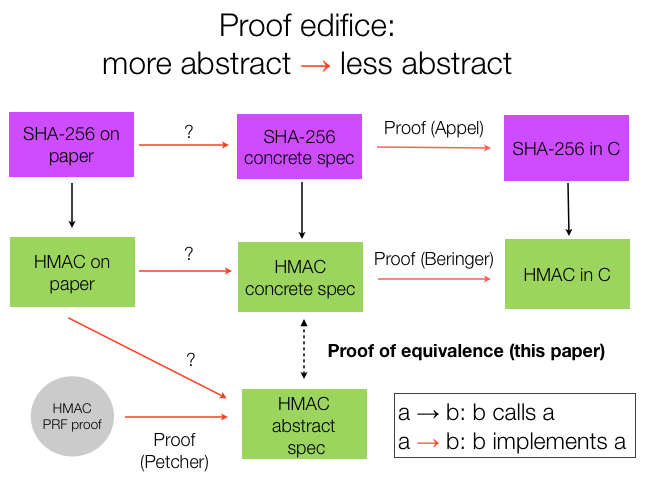
\includegraphics[scale=0.35]{Proof_edifice}
	\caption{Mind the gap (the dotted arrow).}
\end{figure}	

\subsection{Formal verification in Coq}

Coq is a proof assistant in which every proof step is checked by the small, trusted Coq kernel. Among other things, Coq has been used to complete a computer-checked proof of the four-color theorem and to  develop CompCert, a formally verified C compiler.

Coq has two internal languages, Gallina and the tactic language. Gallina is a purely functional language similar to OCaml. The tactic language is used for doing proofs and defining new proof strategies.

As used here, formal verification of a piece of code means proving that this implementation fulfills some kind of high-level specification. The code will usually be written in a low-level language such as C and may contain optimizations and other tricks. The specification, or "spec," will usually be written in a high-level language such as OCaml or Gallina and is typically more mathematical and abstract. A program without a specification {\it cannot be incorrect}, it can only be surprising.\footnote{Paraphrase of J. J. Horning (1982) by Appel (2015).}

% TODO insert VFA code
For example, one may specify that the English description "to be sorted" is equal to the conjunction of two mathematical properties, perhaps specified mathematically in Coq:

\begin{enumerate}
\item The output is a permutation of the input (meaning that no items have been changed, dropped, or added).
\item Each element in the output is less than or equal to all elements to the right, for some definition of $\leq$.
\end{enumerate}

Appel (2014)'s exercises demonstrate this process of formal verification by asking the reader to prove that an implementation of insertion sort in Gallina always satisfies these properties. In the real world, formal verification might entail proving that an optimized implementation of quicksort in C satisfies these properties. 

\subsection{The Merkle-Damg{\aa}rd construction}
% TODO add accent on Damgard
Say we have a strong one-way cryptographic compression function that has been proved to be collision resistant. The problem is that it only operates on an input of a fixed length.

The Merkle-Damg{\aa}rd construction (referred to as "M-D" from now on) is a way to extend this function to inputs of any length by iterating the compression function on identically-sized, adjacent blocks of the input. It has been proven to preserve the collision-resistance property of its internal compression function. M-D has been used to design many popular hash algorithms such as MD5, SHA-1, and SHA-2. 

\begin{figure}[h!]
	\centering
	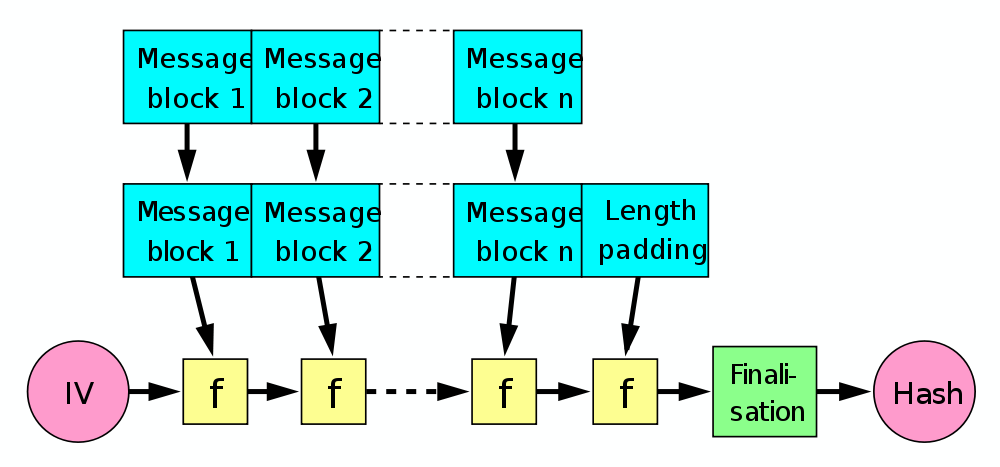
\includegraphics[scale=0.24]{Merkle-Damgard}
	\caption{The Merkle-Damg{\aa}rd construction. $IV$ denotes the initialization vector and $f$ denotes the compression function.}
\end{figure}

Both of Bellare's HMAC proofs (1996, 2006) require that the underlying hash function is a Merkle-Damg{\aa}rd construction on a compression function $f$ such that $f$ is a pseudo-random function. (Another assumption on $f$ is discussed in Section III.)

\subsection{SHA-256}

SHA-256 is a popular cryptographic hash algorithm constructed via Merkle-Damg{\aa}rd.

It operates on a message of any length by padding the message and breaking the result into 512-bit blocks. After iterating its internal compression function on each block, it outputs a 256-bit digest. 

Like all such hash functions, the version of SHA-256 specified in English in FIPS 180-4 comes with guarantees of pre-image resistance, second pre-image resistance, and collision resistance. (Code that implements FIPS 180-4 does not necessarily come with such guarantees unless they are formally proven about the code.) Thus, it is very difficult for an adversary to change the input message without changing the digest. It will be assumed for the HMAC proof that the functional spec of SHA-256 is a pseudo-random function on its inputs; however, nobody knows how to prove that.

\subsection{HMAC}

SHA-256 provides only a guarantee of integrity; that is, a guarantee the message has not been tampered with. A message authentication code (MAC) is used to guarantee both integrity and authenticity, the latter meaning that the message's origin is the expected sender. Sender and receiver need only exchange a secret key before beginning their communication. In addition, whereas SHA-256 is vulnerable to length-extension attacks, HMAC is not.

To accomplish this, HMAC (a "hash-based message authentication code") was designed by Bellare (1996). It includes a proof that the HMAC protocol (described below) is a pseudo-random function (PRF) on its inputs given that the underlying hash primitive is a PRF, a proof which was improved by Bellare (2006). In SHA-256, the underlying hash primitive would be its compression function.
% TODO different MAC security requirements

To compute the authentication code of a message, RFC 2104 defines HMAC as the following action:
$$HMAC_{H, K}(m) = H ( (k \oplus opad) | H ( k \oplus ipad | m )  ) $$

where

\begin{itemize}
\item its block length is 512 bits, or 64 bytes,
\item $H$ is a cryptographic hash function (here, $SHA$-$256$),
\item $K$ is a secret key padded to the right with extra zeros to the input block size of the hash function, or the hash of the original key if it's longer than that block size, 
\item $m$ is the message to be authenticated, 
\item $|$ denotes concatenation, 
\item $\oplus$ denotes bitwise exclusive or (XOR), 
\item $opad$ is the outer padding (the byte $0x5c$ repeated 64 times to be the length of one block), 
\item and $ipad$ is the inner padding ($0x36$ repeated as above).
\end{itemize}

Note that formalizing HMAC is a natural extension of our work on SHA-256, since HMAC is not much more complicated than applying a cryptographic hash function twice. 

OpenSSL includes an implementation of HMAC in C which calls the OpenSSL implementation of SHA-256.

\begin{figure}[h!]
	\centering
	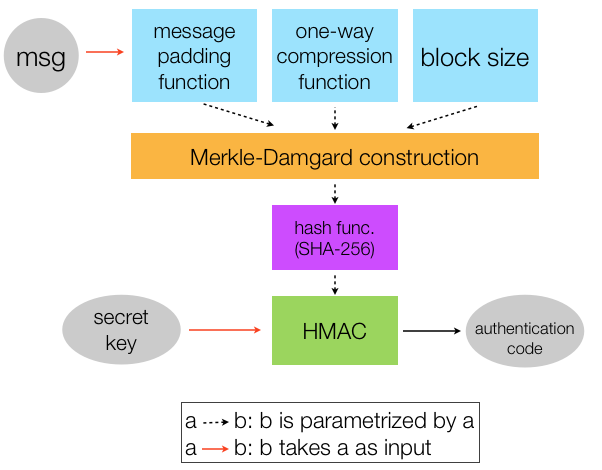
\includegraphics[scale=0.4]{Cryptosystem}
	\caption{The entire system. It is slightly more correct to think of a "black box" HMAC taking message and key as input, and outputting the authentication code.}
\end{figure}

% \subsection{Prior work}

% Verification of SHA-256.

%%%%%%%%%%%%%%%%%%%%%%%%%%%%%%%%%%%%%%%%%%%%%%%%%

\section{Proofs of equality and equivalence}

\subsection{The concrete HMAC spec}

% TODO it is called the concrete spec because...
Beringer (2015) wrote a specification of HMAC to conform to RFC 2104 (IETF's English description of the algorithm); thus, it contains runnable code, operates on byte lists, and returns a byte list. Because the code contains no abstract parameters and can be run as-is, we call it the "concrete" spec. The spec distinguishes between the $Z$ type and the $byte$ type (values of type $Z$ in range $[0, 255]$); however, in this paper, we will use $Z$ synonymously with $byte$ with the understanding that all values are in range.

The spec is constructed to work with generic cryptographic hash functions. We will instantiate it with the $SHA$-$256$ functional program, which the spec treats as a black box that takes care of the message padding and compression function iteration.

The code for this spec and the next is in the Appendix. % TODO note about location of all code

\subsection{The abstract HMAC spec}

% TODO elaborate on Bellare stuff and what exactly they say about it in the paper
% TODO it is called the abstract spec because...
Petcher (2015) wrote a specification of HMAC to conform to the protocol defined by Bellare (1996). Because the code cannot be run until several abstract parameters are instantiated, we call it the "abstract" spec.

To be as general as possible, it operates on bits instead of bytes. Instead of the byte lists used in the concrete spec, it uses bit vectors. (A bit list, or $Blist$, is a list of bits of any length. A bit vector $Bvector \textrm{ } n$ is a type dependent on a natural number value $n$, the length of the vector. $Bvector \s n$ is basically a $Blist$ constrained to be of length $n$, which is checked at compile-time.) The abstract spec uses vectors because Bellare's proof often requires that a list of bits possess a certain length. For example, we translate "$opad$ and $ipad$ are exactly one block long" into code as $(opad \s ipad : Bvector \s b)$.

The abstract spec defines HMAC via the two-keyed HMAC ($HMAC\_2K$) and generalized HMAC ($GHMAC\_2K$) structures, rather than straightforwardly as the concrete spec does. It also includes an implementation of generalized NMAC ($GNMAC$), another structure used in the proof.

\lstinputlisting[lastline=19]{../HMAC_spec_parameters.v}

% TODO code here

Bellare (1996)'s proof, and hence Petcher (2015)'s proof, depend on the following assumptions that are explicit in the spec:
\begin{enumerate}
\item the key is of the right length (one block)
\item $opad \neq ipad$ (they differ in at least one bit)
\item the padding function $splitAndPad$ is one-to-one
\item the hash function (e.g. $SHA$-$256$) is an iterated version of the compression function; that is, it is constructed via Merkle-Damg{\aa}rd.
% TODO a la
\end{enumerate}

as well as other implicit assumptions explained in Section III.

The fourth assumption can be seen in this definition of the $SHA$-$256$ analogue, $hash\_words$:

\lstinputlisting[firstline=23, lastline=28]{../HMAC_spec_parameters.v}

However, $SHA$-$256$ includes a padding function for the message, while this spec's use of dependent types ($Bvector \textrm{ } n$) forces the use of two types of ad-hoc padding, the functions $app\_fpad$ and $splitAndPad$. 

\lstinputlisting[firstline=55, lastline=59]{../HMAC_spec_abstract.v}

\lstinputlisting[firstline=112, lastline=113]{../HMAC_spec_parameters.v}

\lstinputlisting[firstline=115, lastline=116]{../HMAC_spec_parameters.v}

$fpad$ is used to pad the output size $c$ to the block size $b$. $splitAndPad$ is used to split the variable-length message (of type $Blist$) into a list of blocks, each size $b$, padding it along the way.

\subsection{Proof outline}

There are six main differences between the concrete and abstract specs:
\begin{enumerate} 
\item the abstract spec operates on bit lists, whereas the concrete spec operates on byte lists.
\item the abstract spec uses the dependent type \verb|Bvector n|, which is a bit list of length $n$, whereas the concrete spec uses byte lists and int lists.
\item due to its use of dependent types, the abstract spec pads its input twice in an ad-hoc manner, whereas the concrete spec uses the SHA-256 padding function consistently.
\item the concrete spec treats the hash function (SHA-256) as a black box, whereas the abstract spec exposes various parts of its functionality, such as its initialization vector, internal compression function, and manner of iteration. (It does this because the Bellare proofs require that the hash function is constructed via Merkle-Damg{\aa}rd.)
\item the abstract spec does an explicit fold over the message, which is now a list of blocks, not a list of pure bits.
\item the abstract spec defines HMAC via the HMAC\_2K and GHMAC\_2K structures, not directly. 
\end{enumerate}

\begin{figure}[h!]
	\centering
	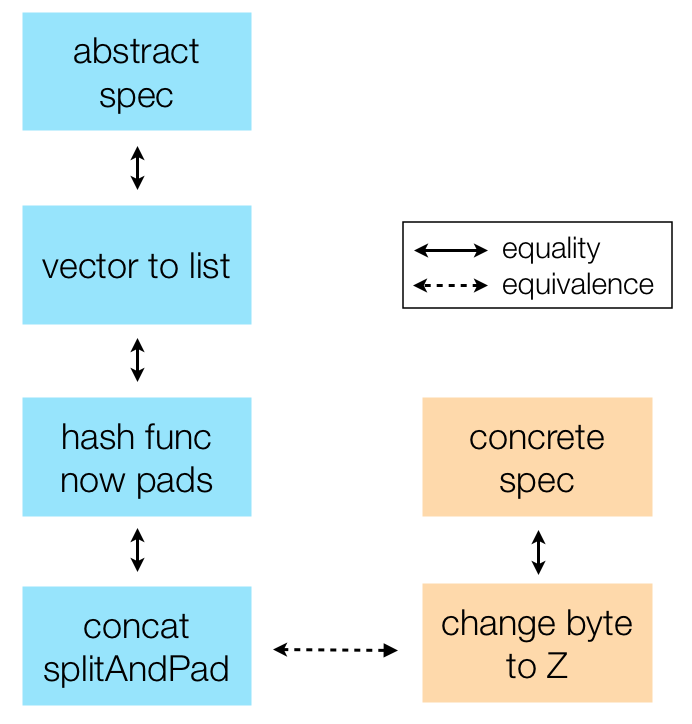
\includegraphics[scale=0.56]{Equivalence_proof_chain}
	\caption{Stages of the equivalence/equality proofs.}
\end{figure}

% TODO reorder these
They are ranked in rough order of most difficult to least difficult. 
% No difficulty is too great to be overcome--we believe the specs are not "fundamentally different" and that they can be linked via proof. Indeed, a goal of this project was to find and remove differences in the process of proof.

The last, $6$, is easily resolved by unfolding the definitions of HMAC\_2K and GHMAC\_2K. We solve the other five by changing definitions and massaging the two specs in the "same direction," proving equality each time.

$5$ is resolved by concatenating the $list \s(Bvector \s b)$ in $hash\_words$ below. Then it can be seen that iterating $firstn \s b$ and $splitn \s b$ over the concatenated list is equal to left-folding over the list of blocks.

\lstinputlisting[firstline=94, lastline=102]{../HMAC_spec_parameters.v}

\lstinputlisting[firstline=104, lastline=108]{../HMAC_spec_parameters.v}

$4$ is not too difficult. Its explicit fold (as iteration method) can be proven equal to the iteration method using $firstn$ and $splitn$ in the concrete SHA-256 spec, as seen in $3$ above. It suffices to convert the SHA\_256 initialization vector and wrap its internal compression function. See $1$ and the next section for an elaboration on conversion and wrapping.

Before iterating the compression function on the message, SHA-256 pads it in a standard, one-to-one fashion so its length is a multiple of the block size. It pads it as such:
\eqn{msg\s | \s [1] \s | \s [0, 0, \ldots 0] \s | \s [l_1, l_2]}

where $|$ denotes concatenation and $[l_1, l_2]$ denote the two digits of the length of the message as a 64-bit integer. The number of $0$s is calculated such that the length of the entire padded message is a multiple of the block size. 

 Thus, $3$ is resolved by rewriting the abstract spec to incorporate $fpad$ and $splitAndPad$ into a single padding function included in the hash function, much like SHA-256 does.
\eqn{ hash\_words\_padded := \\ hash\_words \circ split\_and\_pad}

As summarized in the previous section, $fpad$ is used to pad the output size $c$ to the block size $b$. $splitAndPad$ is used to split the variable-length message (of type $Blist$) into a list of blocks, each size $b$, padding it along the way. $fpad$ is instantiated as a constant, since we know that the length of the message is $c < b$. $splitAndPad$ is instantiated as the normal SHA padding function, but tweaked to add one block size to the length appended in $[l_1, l_2]$, since $k_{in}$ (with a length of one block) will be pre-pended to it later.\footnote{Bellare (1996) glosses over the padding methods: "Notice that a way to pad messages to an exact multiple of b bits needs to be defined (...) SHA pad[s] inputs to always include an encoding of their length" (8). The process of formalizing proofs in code dispels the vagueness that hides in natural language. }

$2$ is resolved by changing all $Bvector \s n$ to $Blist$, then proving that all functions preserve the length of the list when needed. This maintains the $Bvector \s n$ invariant that its length is always $n$.

$1$ is the most difficult; since the types of each HMAC function differ, it requires an equivalence proof rather than an equality proof. It is discussed in the next section. 

% A minor difference also exists between the SHA-256 concrete spec, which uses the $Z$ type, and the HMAC concrete spec which uses the $byte$ type (range-constrained $Z$). This is resolved by asserting and proving that $\forall x:Z, x \in [0, 255]$ wherever needed.

%%%%%
\subsection{Bridging bytes and bits}

We would like to prove that the concrete and abstract HMAC specs ($HMAC_c$ and $HMAC_a$) are extensionally equal. That is, equal inputs always result in equal outputs: 
\begin{gather*}
k_c = k_a \rightarrow \\
m_c = m_a \rightarrow \\
HMAC_c(k_c, m_c) = HMAC_a(k_a, m_a).
\end{gather*}

However, $HMAC_c$ operates on bits (in fact, vectors of bits) and $HMAC_a$ operates on bytes (lists of bytes). So the statement $k_c = k_a$ (for example) does not have meaning because the types are different. To solve this, we generalize equality to equivalence. Given that the inputs are {\it equivalent}, the outputs will be {\it equivalent}.
\begin{gather*}
k_c \approx  k_a \rightarrow \\
m_c \approx m_a \rightarrow \\
HMAC_c(k_c, m_c) \approx HMAC_a(k_a, m_a).
\end{gather*}

The equivalence relation $\approx$ can be defined either computationally or inductively. Both definitions will turn out to be useful. (From now on, we will use $b$ to name a value of type $Blist$ (list of booleans, or bits) and $B$ to name a value of type $list$ $Z$ (list of bytes).)

The computational relation is 
\begin{gather*}
b \approx_c B := \\
b = bytesToBits \textrm{ } B,
\end{gather*} where $bytesToBits : list \textrm{} Z \rightarrow Blist$ is a conversion function.

% TODO explain inductive
The inductive relation is 
\begin{gather*}
b \approx_i B := \\
bytes\_bits\_lists \textrm{ } b \textrm{ } B.
\end{gather*}

where $bytes\_bits\_lists : Blist \rightarrow list \textrm{ } Z \rightarrow Prop$ creates an "assertion" that $b$ and $B$ are related in this way, together with two constructors used to provide evidence to prove the assertion. (For more on inductively defined propositions, see the $Prop$ chapter in the Coq textbook "Software Foundations" (Pierce et al. (2014)).)

% TODO fix formatting, maybe embed inline
\lstinputlisting[firstline=27, lastline=34]{../ByteBitRelations.v}

The inductive and computational definitions have been proven equivalent in the sense that 
$$bytes\_bits\_lists \textrm{ } b \textrm{ } B \leftrightarrow b = bytesToBits \textrm{ } B.$$

For several other ways to convert between the definitions, see $ByteBitRelations.v$ in the \texttt{vst-hmac} distribution linked in the Introduction.

% Insert abstract section here

\subsection{Instantiating the abstract specification}

We instantiate the block sizes and wrap the concrete functions in $byteToBit$ and/or $intlist\_to\_Zlist$ conversion functions. The latter is necessary because portions of the SHA-256 spec operate on lists of $Integer$s, as specified in FIPS 180-4.\footnote{Actually, FIPS 180-4 defines SHA-256 on a bitstring of any length, similar to the Bellare proof. But OpenSSL's implementation permits only sequences of bytes; that is, multiples of 8 bits.} ($Z$ in Coq denotes arbitrary-precision mathematical integers. The SHA-256 spec uses $Z$ to denote bytes. An $Integer$ is four $Z$ packed big-endian into a 32-bit integer.)

\lstinputlisting[firstline=32, lastline=48]{../HMAC_spec_parameters.v}

Note that we are essentially converting the type of the values from $intlist \rightarrow \ldots \rightarrow intlist$ to $Blist \ldots \rightarrow \ldots Blist$ by converting their inputs and outputs.

We can use the computational equivalence relation defined earlier ($\approx_c$), instantiated with a generic conversion function, to reason abstractly about the behavior of such wrapped functions. Let's define the framework as such (letting $. = \circ$, function composition):

\lstinputlisting[firstline=52, lastline=58]{../HMAC_spec_parameters.v}

Note that the types $B$ and $A$ are not symmetric, in the sense that 

Define two relations as such:
\eqn{
x \approx_c X := \\
x = convert\_BA \textrm{ } X.
}
\eqn{
f \approx_w F := \\
f = wrap \textrm{ } F.
}

We ask: what assumptions are needed such that application of equivalent (via wrapping) functions to equivalent (via conversion) inputs result in equivalent (via conversion) outputs?
\eqn{
Lemma \spc once\_eq : \\
\forall \spc (x : A) \spc (X : B) \spc (f : A \rightarrow A) \spc (F : B \rightarrow B),\\
x \approx_c X \rightarrow \\
f \approx_w F \rightarrow \\
f \spc x \approx_c F \spc X
}

The necessary and sufficient assumption (together with the other two assumptions) is that we have output equivalence exactly when a "round-trip" of composing the two conversion functions results in the identity function. (The reader is invited to finish this short proof.)
\eqn{
Lemma \spc roundtrip : convert\_AB \circ convert\_BA = id }

Indeed, we have proven that $bitsToBytes \circ bytesToBits = id$. Note that it does not hold the other way around. $bytesToBits \circ bitsToBytes$ is false if the length of the bit list input is not a multiple of 8.

A natural extension is to prove output equivalence on repeated application of the wrapped functions, or iteration:

\lstinputlisting[firstline=78, lastline=82]{../HMAC_spec_parameters.v}
\eqn{
Lemma \spc iterate\_equiv : \\
  \forall  \spc (x : A) \spc (X : B)\\
   (f : A \rightarrow A) \spc (F : B \rightarrow B) \spc (n : nat), \\
    x \approx_c X \rightarrow \\
    f \approx_w F \rightarrow \\
    iterate \spc n \spc f \spc x = convert\_BA \spc (iterate \spc n \spc F \spc X).
}

Here we need both $once\_eq$ and our newly admitted assumption $roundtrip$, which can be rephrased as $\forall (X : B), X = roundtrip \spc X$. The proof is completed by induction on $n$.

This framework is not just an academic exercise. $once\_equiv$ and $iterate\_equiv$ correspond directly to several lemmas in the bytes/bits equivalence proof. In particular, $iterate$ corresponds directly to the SHA-256 operation of hashing blocks. 

\lstinputlisting[firstline=178, lastline=182]{../SHA256.v}

The proof of equivalence works the same way. One can almost directly substitute the parameters into $iterate\_equiv$. 
\eqn{
Lemma \s fold\_equiv\_blocks : \\
\forall (l : Blist) \s (acc : Blist) \s (L : list \s int) \s (ACC : list \s int), \\
      InBlocks \s 16 \s L \rightarrow \\
      l \approx_c L \rightarrow \\
      acc \approx_c ACC \rightarrow \\
      hash\_blocks\_bits \s sha\_h \s acc \s l \s \approx_c SHA256.hash\_blocks \s ACC \s L.
}	

The only differences are that the functions in question take multiple inputs, the length of $L$ must be a multiple of 16 (the block size for the $Integer$ type, 512 bits), and the method of iteration is slightly modified to be parametrized by the length of the input list ($firstn$, $skipn$). $sha\_h$ contains the wrapped $SHA256.hash\_block$ function. $hash\_blocks\_bits$ is a version of $SHA256.hash\_blocks$ modified to use 512 as its block size. The code for the proof is in $HMAC\_spec\_concat.v$.

One wonders whether this "one-way roundtrip" property has been formalized elsewhere, perhaps in a Coq abstract algebra library. We found that the concepts of Galois connections and setoids were similar, but not useful.

In sum, the computational relation $\approx_c$ makes abstract reasoning easy precisely because it is computational, so one can rewrite using equality in proofs. If no conversion function existed, one could use the inductive relation $x \approx_iX$, but it does not easily allow rewrites, since $x$ and $X$ are of different types. The strength of $\approx_i$ will be discussed in the next section.

\subsection{The proof of equivalence}

The main equivalence theorem is as follows. The symbol $\approx$ will be used to represent either relation ($\approx_c, \approx_i$) interchangeably. 
\eqn{
Theorem \s HMAC\_spec\_equiv : \\
\forall
                            (k \s m \s h : Blist) (op \s ip : Blist) \\
                            (K \s M \s H : list \s Z) (OP \s IP : list \s Z), \\
  length \s K = SHA256.BlockSize \rightarrow \\
  k \approx K \rightarrow \\
  m \approx M \rightarrow \\
  op \approx OP \rightarrow \\
  ip \approx IP \rightarrow \\
  HMAC \s c \s p \s sha\_h \s sha\_iv \s sha\_splitandpad \s op \s ip \s k \s m = h \rightarrow \\
  HMAC\_SHA256.HMAC \s IP \s OP \s M \s K = H \rightarrow \\
  h \approx H.
}

Note that the following are implicit: 
\eqn{
	sha\_iv \approx_c SHA256.init\_registers \\
	sha\_h \approx_w SHA256.hash\_block \\
	sha\_splitandpad \approx_w sha\_padding\_lemmas.pad
}

$sha\_padding\_lemmas.pad$ is a version of $SHA256.generate\_and\_pad$, the padding function defined in FIPS 180-4, modified here to separate the padding from the $Z \rightarrow Integer$ conversion. $hash\_blocks\_bits$ is a version of $SHA256.hash\_blocks$ modified to use 512 as its block size. 	

As a refresher, here is the HMAC code:
$$HMAC_{H, K}(m) = H ( (k \oplus opad) | H ( k \oplus ipad | m )  ) $$
% bits
% $$HMAC_{H, K}(m) = H ( (k \oplus opad) | H ( k \oplus ipad | m )  ) $$

Section IIc discussed the series of transformations applied to the abstract spec. Its structure was originally not close to the HMAC and SHA code, but after some massaging, it and its internal hash function become structurally similar enough to the high-level code for the proof to be  decomposed by function.

Three functions occur in the definition of HMAC: \\ $H$ (hashing), $|$ (concatenation), and $\oplus$ (bitwise xor). Thus, the proof breaks up naturally and modularly into three theorems. For each function, its theorem states that the output is equivalent given that the input is equivalent. 
\eqn{
Lemma \s f\_equiv : \forall (b : bits) (B : bytes), \\
b \approx B \rightarrow  \\
f \approx_w F \rightarrow \\
f \spc b \approx F \spc B.}

The proof is completed by backward-chaining these implications. The diagram makes it clear that in the end, the leaves of the tree are the sole propositions that need to be proved, and these are exactly the givens: $k \approx K, m \approx M, op \approx OP,$ and $ip \approx IP$.

% TODO inline graphic
 \begin{figure}[h!]
 	\centering
 	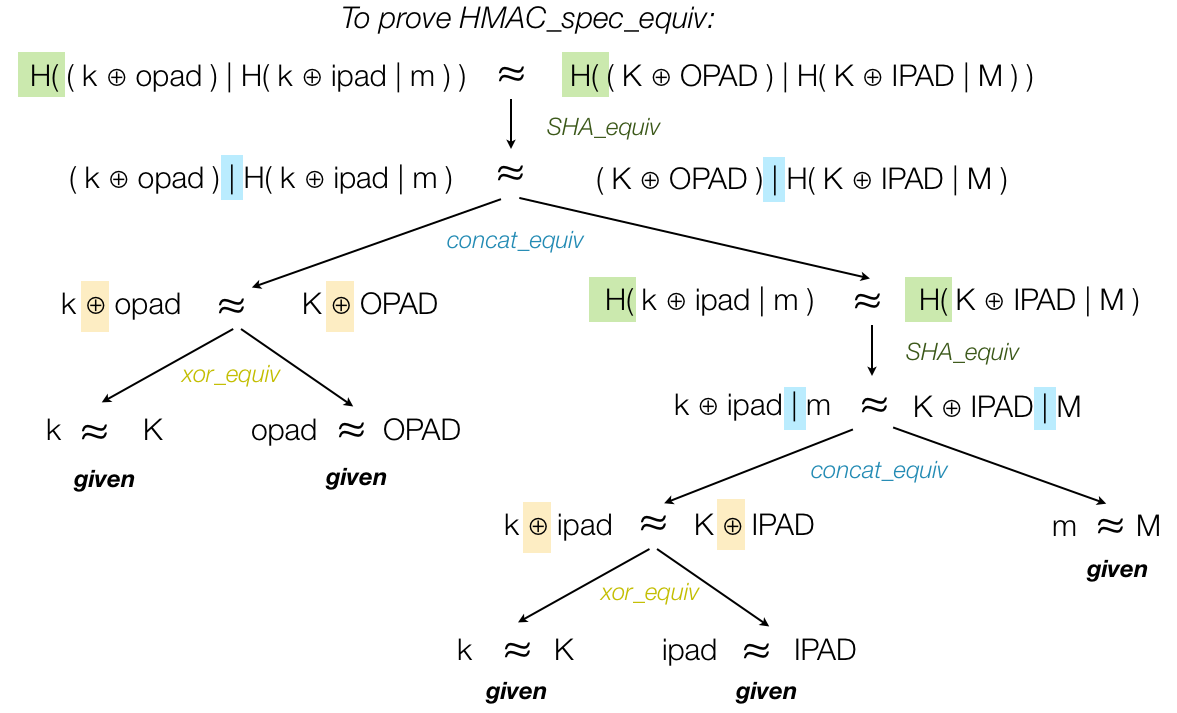
\includegraphics[scale=0.21]{HMAC_spec_equiv}
 	\caption{$a \xrightarrow{T} b$ means "By $T$, $b$ implies $a$." Note after HMAC has been unpacked, all that is left is our assumptions.}
 \end{figure}

The theorem about $|$, $concat\_equiv$, is easy to prove by induction. \\
\indent
The theorem about $\oplus$, $xor\_equiv\_Z$, is slightly harder. It uses the inductive relation and depends on several lemmas in $XorCorrespondence$, including a large proof by brute force. The proofs use the inductive relation $\approx_i$ because it comes with a stronger induction principle that allows us to break up the input bit/byte lists correctly to perform induction, since eight bits correspond to one byte.
\indent

Lastly, the theorem about $H$, $SHA\_equiv\_pad$, depends on $fold\_equiv$. $fold\_equiv$ requires a messy double induction that requires definition and use of the $InBlocks \s n$ inductive proposition. This is necessary because one list is in blocks of 512 bits and the other is in blocks of 16 integers.

In addition to the main theorems, the equivalence proof involves about 45 more lemmas.

\subsection{Other proof techniques}

The following techniques may be useful for future Coq developments.

Many theorems are true for lists of any length (e.g. some involving map and zip). We found it difficult to do induction on $Bvector \s n$, dependent type induction, since its length is fixed. Instead, we found it easy to prove theorems by induction on a Blist, implying that the list may be any length, then specialize it to \verb|Bvector n|, a Blist of length $n$. 

Likewise, we found it easier to prove theorems about lists of any length (or a certain length given by an assumption), then prove that the functions involved preserve the length. This is equivalent to working with \verb|Bvector n|. % TODO add examples

When dealing with lists whose lengths must be a multiple of a block size (e.g. 512 bits or 64 bytes), we found it useful to define an inductive proposition $InBlocks \s n$ that would allow one to do proofs by inducting in the block size, cons'ing elements to the front. This allows an easier induction on bit/byte lists, since 512 bits correspond to 64 bytes. We then proved $InBlocks \s n$ equivalent to the computational version (using the length function). % code here

Likewise, we found it useful to define both inductive and computational definitions, as covered in the previous sections: a function to compute conversions between byte lists and bit lists, and an inductive proposition stating the existence of bits such that the two lists correspond.

When it comes to theorems that involve tricky math, we exploited the fact that range of a byte is $[0, 255]$ and proved them by brute force instead. The same technique also works in reverse. Proving something true for $8$ booleans is as simple as checking that the statement is true for each of the $256$ cases. % code here

\subsection{Problems encountered}

Initially, we attempted to do the proof on the abstract spec as-is. We found it difficult to work with dependent types, induction, and John Major equality (McBride (2002)), which is a generalization of equality necessary to deal with dependent types. One common problem was that there are no easy Coq facilities for type-level manipulation, e.g. Coq cannot automatically convince itself that $\forall (n : nat), \s Bvector \s (n+1) = Bvector \s (S \s n)$. This crops up often in recursive functions.

Additionally, we encountered problems converting between many machine representations of numbers: byte and bit of course, byte and Z, integer and Z, and even little-endian and big-endian.

Lastly, we did not find much prior work on this sort of equivalence proof or the "one-way roundtrip" algebraic property, except for related functions in Coq.Strings.Ascii (Thery).

\section{The proof of HMAC's security}

\subsection{The 1996 Bellare proof}

Let $f$ be the compression function and $f^*$ the iteration of $f$ (i.e. something like SHA-256, constructed via the Merkle-Damg{\aa}rd construction).

Given the assumption that $f$ is a pseudo-random function (PRF), that implies that $f^*$ is computationally almost universal ($cAU$). $cAU$ is a slightly weaker property than collision-resistant (Bellare (1996) uses collision-resistance; Bellare (2006) weakens it to $cAU$.) An RKA is a related-key attack wherein the adversary queries the function both with the target key and with other adversary-defined keys. The adversary may know that there is some mathematical relationship among the keys, but might not know the exact value of the keys.

% (\verb|goo.gl/wK8OXg|)
\begin{figure}[h!]
	\centering
	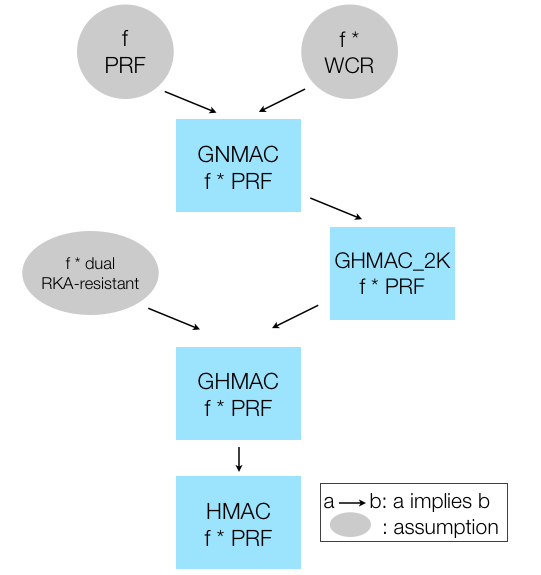
\includegraphics[scale=0.4]{HMAC_proof}
	\caption{The structure of the 1996 Bellare HMAC proof.}
\end{figure}

(Among other simplifications, Bellare (2004) proves that the $f \s PRF$ assumption implies the $f^* \s cAU$ assumption, indicated by the dotted arrow in Figure 6. (TODO))

The $f^* cAU$ property is used to prove that generalized NMAC (GNMAC) using $f^*$ is a PRF. The GNMAC property is used to prove that generalized HMAC with two keys (GHMAC\_2K) using $f^*$ is a PRF.

Using that fact and the assumption that $f^*$ is RKA-resistant, we prove that GHMAC (single-keyed) using $f^*$ is a PRF. This, plus the fact that the padding function for $f$ is one-to-one, leads finally to the proof that HMAC using $f^*$ is a PRF.

%%%%%%%%%%%%%%%%%%%%%%%%%%%%%%%%%%%%%%%%%%%%%%%%%

\subsection{Formalization in Coq}

Petcher (2014) presents the "Mechanized Cryptography Framework," a probabilistic programming language implemented in Coq. Petcher (2015) formalizes Bellare's 1996 proof using MCF. (TODO)

\subsection{Transfer of properties}

In order for the the proof to hold, the following assumptions must hold:
\begin{itemize}
\item the splitAndPad function is one-to-one (that is, $pad(m_1) = pad(m_2) \rightarrow m_1 = m_2$).
\item opad and ipad differ in at least one bit.
\item $f$ is a pseudo-random function.
\item $f^*$ is resistant to related-key attacks.
\item Appel (2015)'s concrete spec of SHA-256 is a Merkle-Damg{\aa}rd construction.
\end{itemize}

Examining the final spec, these are mostly true. It is obvious on inspection that the SHA padding function, and thus the wrapped SHA padding function, are one-to-one. Beringer (2015) also defined $opad$ and $ipad$ to be different. However, it is unknown whether $f$ (the internal SHA compression function) is a PRF--this is an open conjecture. Also, we have not been able to determine whether SHA-256 is resistant to related-key attacks. (TODO) The last item is provable and is left as future work.

% TODO future work
Thus, via the $PRF\_Convert$ argument, the following theorem can be stated: "there exists a function $f$ that is equivalent to the C program, and $f$ is a pseudo-random function." (TODO, unclear)

After composing the theorems, the HMAC specs "drop out" of the proof, leaving an end-to-end proof of correctness.

\subsection{The HMAC brawl}

(TODO: should I summarize this and the last two sections in more detail, or leave it to the joint paper?)

\section{conclusion}

% TODO rewrite 
Again, we bridge the gap between the abstract and the concrete HMAC spec by formally proving their equivalence. This proof transfers the desirable and necessary property of being a pseudo-random function (with some caveats) to both the concrete spec and the C implementation of HMAC, guaranteeing that the OpenSSL code provides cryptographic security (as specified by Bellare (1996)).

We also contribute a theory of reasoning about equivalence, especially between programs working with bytes and programs working with bits. We formalize the theory in a small library for reasoning about these correspondences and converting between inductive and computational definitions.

We have also added comments on our success or failure using general Coq proof techniques, including brute force, dependent types, and inductive propositions for length ($InBlocks \s n$).

Lastly, we have not entered the ring of the HMAC brawl, but we present our chain of successful formalizations in hopes that they are valuable to cryptographers interested in computer-checked proofs of correctness. Additionally, the security guarantees on the OpenSSL HMAC implementation resulting from our work are still strong enough for practical use. (TODO, vague)

\subsection{Future work}

We would like to compose the various proofs (Figure 1) to leave an end-to-end proof of correctness. This requires more work: we need to enumerate and/or prove various assumptions made in the course of constructing the system, then state exactly which properties of security transfer to the C program. For example, it is still necessary to prove that Appel (2015)'s concrete spec of SHA-256 is a Merkle-Damg{\aa}rd construction. 

In the fields of formal verification and programming languages, more libraries could be written to aid reasoning about equivalence and lengths, as well as facilitate type-level programming in Coq. We anticipate that future work bridging paper proofs with code will run into many of the same problems that we did.

In the field of cryptography, much interesting work is being done now on techniques, frameworks, and formalization of cryptographic protocols and algorithms. EasyCrypt (Backes (2012)), CertiCrypt (Barthe (2009)), and MCF (Petcher (2014)) are all inspired by Bellare, Rogaway, and Halevi's vision of code-based, game-based, computer-checked proofs. Of course, the question of whether SHA-256's compression function is a pseudo-random function is yet unresolved.

Lastly, for secure and practical use of HMAC (say, in a military setting) or any symmetric protocol, one needs a secure method of transmitting the secret key between two agents. To that end, it is desirable to formalize, check, and prove security of an implementation of a asymmetric cryptographic algorithm such as RSA.

\begin{acknowledgments}

I would like to thank my advisor, Andrew Appel, for lots of patience, help with Coq hacking, and suggesting this interesting and important project in the first place. I owe a lot to Lennart Beringer for his help with proofs during many weekend meetings.

Adam Petcher deserves thanks for his patience with my many questions about his HMAC spec, and for explaining to me the Bellare proof and his mechanization. Qinxiang Cao helped me realize that several of my proof techniques at that time would not work, and suggested a new idea.

\end{acknowledgments}

% \subsection{References}

 \bibliographystyle{plainnat}

\begin{thebibliography}{99}

  %\emph{\LaTeX: a document preparation system}
  % TODO this style doesn't work for \citet(appel2015} 
  % but BibTeX doesn't seem to work nicely with TeXShop (and both styles introduce a horizontal line)
 
\bibitem{appel2015}
Appel, Andrew W. "Verification of a Cryptographic Primitive: SHA-256." In \emph{ACM Transactions on Programming Languages and Systems (TOPLAS)}, 2015. 

\bibitem{vfa}
Appel, Andrew W. "Verified Functional Algorithms." Oregon Programming Languages Summer School. June 2014. Accessed January 2, 2015.

\bibitem{backes2012}
Backes, Michael, Gilles Barthe, Matthias Berg, Benjamin Gr�goire, C�sar Kunz, Malte Skoruppa, and Santiago Zanella B�guelin. "Verified security of Merkle-Damg�rd." In \emph{Computer Security Foundations Symposium (CSF)}, 2012 IEEE 25th, pp. 354-368. IEEE, 2012.

\bibitem{barthe2009}
Barthe, Gilles, Benjamin Gr�goire, and Santiago Zanella B�guelin. "Formal certification of code-based cryptographic proofs." In \emph{Proceedings of the 36th annual ACM SIGPLAN-SIGACT symposium on Principles of programming languages (POPL),} pp. 90-101. 2009.

\bibitem{bellare2006}
Bellare, Mihir. "New proofs for NMAC and HMAC: Security without collision-resistance." In \emph{Advances in Cryptology--CRYPTO 2006}, pp. 602-619. Springer Berlin Heidelberg, 2006.

\bibitem{bellare1996}
Bellare, Mihir, Ran Canetti, and Hugo Krawczyk. "Keying hash functions for message authentication." In \emph{Advances in Cryptology--CRYPTO 1996}, pp. 1-15. Springer Berlin Heidelberg, 1996.

\bibitem{bellare_games2004}
Bellare, Mihir, and Phillip Rogaway. "Code-Based Game-Playing Proofs and the Security of Triple Encryption." \emph{IACR Cryptology ePrint Archive 2004} (2004): 331.

\bibitem{beringer2015}
Beringer, Lennart. Untitled (stand-in reference for paper on verifying correctness of OpenSSL HMAC code). In progress, 2015.

\bibitem{hmacbrawl}
Bernstein, Daniel J. "The HMAC brawl." Lecture, \emph{Fast Software Encryption (FSE) Rump Session}, March 20, 2012.

\bibitem{cpdt}
Chlipala, Adam. "Certified programming with dependent types" (2014).

\bibitem{fips1804}
FIPS, PUB. "180-4, Secure Hash Standards, Federal Information Processing Standards Publication." Information Technology Laboratory, National Institute of Standards and Technology, Gaithersburg, MD (2008): 20899-8900.

\bibitem{halevi2005}
Halevi, Shai. "A plausible approach to computer-aided cryptographic proofs." \emph{IACR Cryptology ePrint Archive 2005} (2005): 181.

\bibitem{koblitz2013}
Koblitz, Neal, and Alfred Menezes. "Another look at HMAC." \emph{Journal of Mathematical Cryptology 7}, no. 3 (2013): 225-251.

\bibitem{rfc2104}
Krawczyk, Hugo, Mihir Bellare, and Ran Canetti. "RFC 2104: HMAC: Keyed-hashing for message authentication." 1997.

\bibitem{mcbride2002}
McBride, Conor. "Elimination with a motive." In \emph{Types for proofs and programs}, pp. 197-216. Springer Berlin Heidelberg, 2002.

\bibitem{openssl_hmac}
OpenSSL HMAC Documentation. Accessed January 2, 2015. https://www.openssl.org/docs/crypto/hmac.html.

\bibitem{petcher2014}
Petcher, Adam. "The Mechanized Cryptography Framework." Currently unpublished, 2014.

\bibitem{petcher2015}
Petcher, Adam. Untitled (stand-in reference for paper on Bellare proof mechanization). In progress, 2015.

\bibitem{sf}
Pierce, Benjamin C., Chris Casinghino, Marco Gaboardi, Michael Greenberg, Catalin Hritcu, Vilhelm Sjoberg, and Brent Yorgey. "Software foundations" (July 2014).

\bibitem{ascii}
Thery, Laurent. Library Coq.Strings.Ascii. Accessed January 2, 2015. 

% TODO: setoid rewrite, galois connection

\end{thebibliography}

%%%%%%%%%%%%%%%%%%%%%%%%%%%%%%%%%%%%%%%%%%%%%%%%%

\section{appendix}

% TODO syntax highlighting and nicer font
\subsection{The abstract HMAC spec}

\lstinputlisting{../HMAC_spec_abstract.v}

\subsection{The concrete HMAC spec}

\lstinputlisting[lastline=90]{../HMAC_functional_prog.v}

\subsection{Definitions}

\lstinputlisting[firstline=173, lastline=190]{../HMAC_spec_harvard_concat.v}

\lstinputlisting[firstline=20, lastline=24]{../ByteBitRelations.v}

\lstinputlisting[firstline=27, lastline=34]{../ByteBitRelations.v}

% TODO realign code
\subsection{The equivalence proof}

\lstinputlisting[firstline=887]{../HMAC_spec_harvard_concat.v}

\subsection{Other theorems and proofs}

See the repository at \\ \verb|github.com/hypotext/vst-hmac|.


\end{document}